\chapter{Application Layer}

\section{Application Layer Protocols}
\begin{minipage}[t]{0.6\textwidth}
   \subsection{HTTP (Hypertext Transfer Protocol)}
   Used for transferring hypertext requests and information between web browsers and web servers. It forms the basis of communication for the World Wide Web.
   
   \subsection{HTTPS (Hypertext Transfer Protocol Secure)}
   A secure version of HTTP that incorporates encryption and authentication mechanisms provided by SSL/TLS protocols for secure communication over the internet.
\end{minipage}%
\hfill%
\begin{minipage}[t]{0.3\textwidth}
   \begin{figure}[H]
      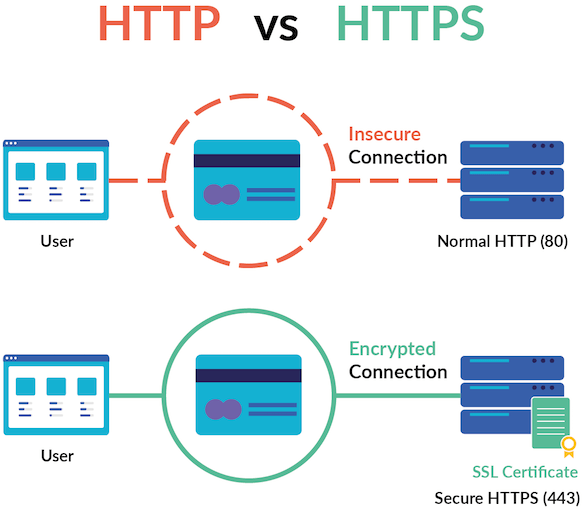
\includegraphics[width=\linewidth]{figures/HTTP and HTTPS.png}
   \end{figure}
\end{minipage}


\subsection{FTP (File Transfer Protocol)}
Enables the transfer of files between a client and a server on a network. It allows users to upload, download, list, rename, and delete files on remote servers.

\begin{figure}[H]
   \centering
   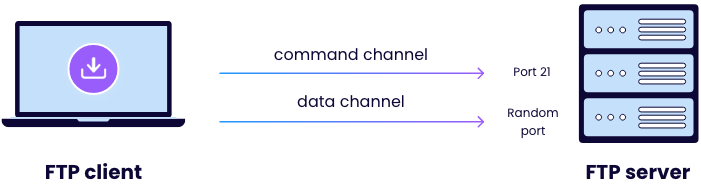
\includegraphics[width=0.6\linewidth]{figures/FTP.png}
\end{figure}

\subsection{SMTP (Simple Mail Transfer Protocol):}
Used for sending email messages between email servers. It defines how email messages are transferred and routed across networks.

\subsection{POP3 (Post Office Protocol version 3):}
Allows email clients to retrieve email messages from a remote server. It is commonly used for downloading emails to the client's device.

\begin{figure}[H]
   \centering
   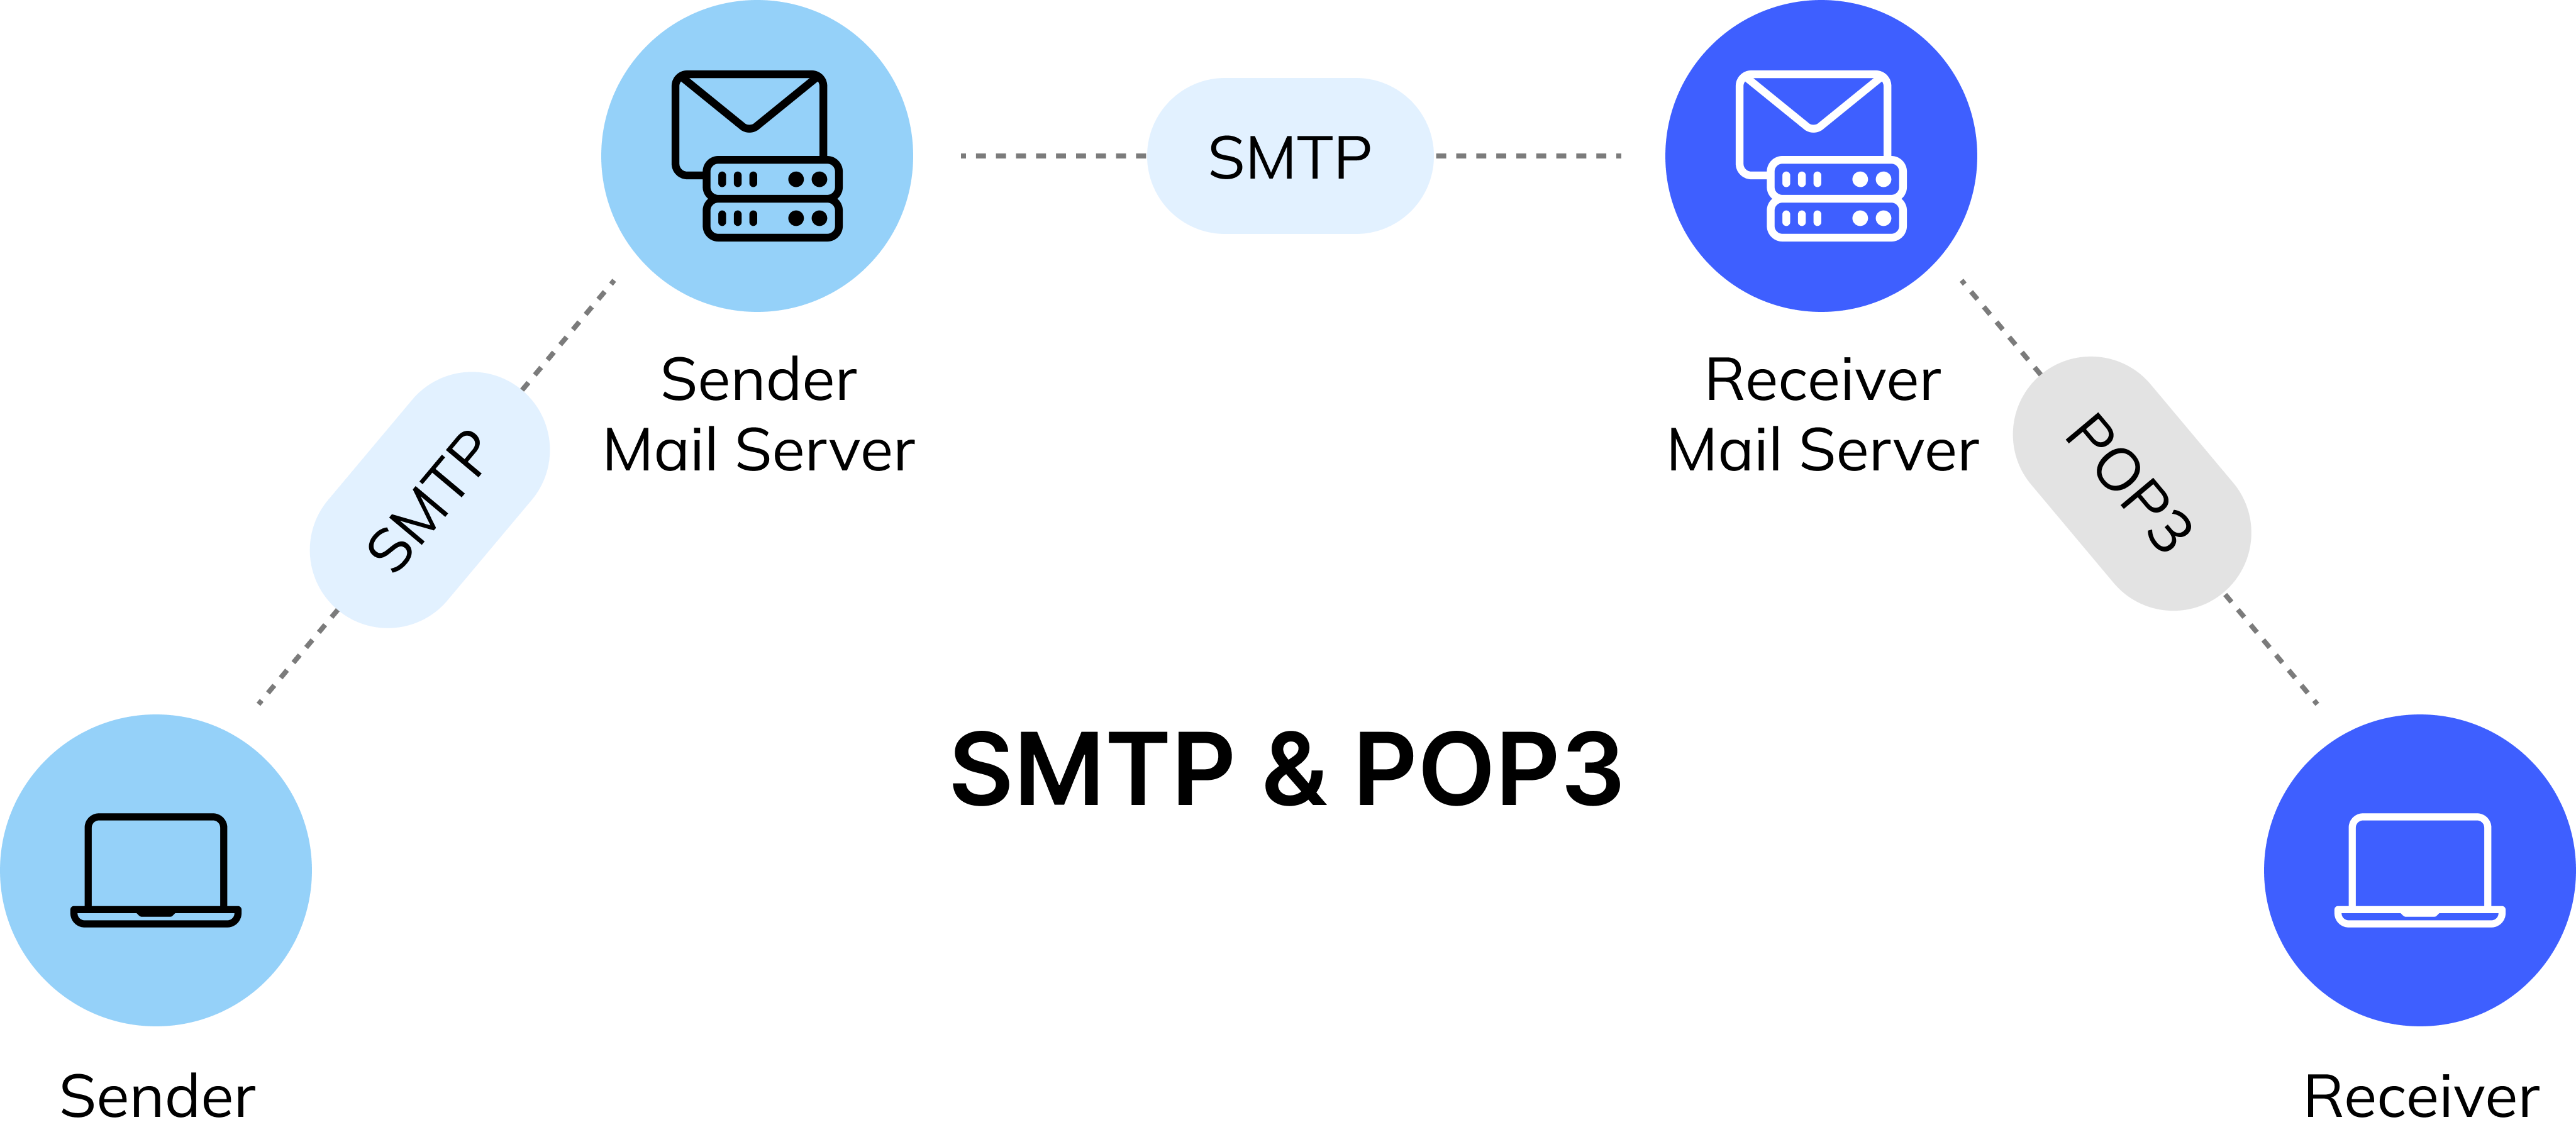
\includegraphics[width=0.6\linewidth]{figures/SMTP.png}
\end{figure}


\section{DNS (Domain Name System):}
Resolves domain names to IP addresses and vice versa. It translates human-readable domain names (e.g., www.example.com) into numerical IP addresses used by computers to communicate over a network.

\begin{figure}[H]
   \centering
   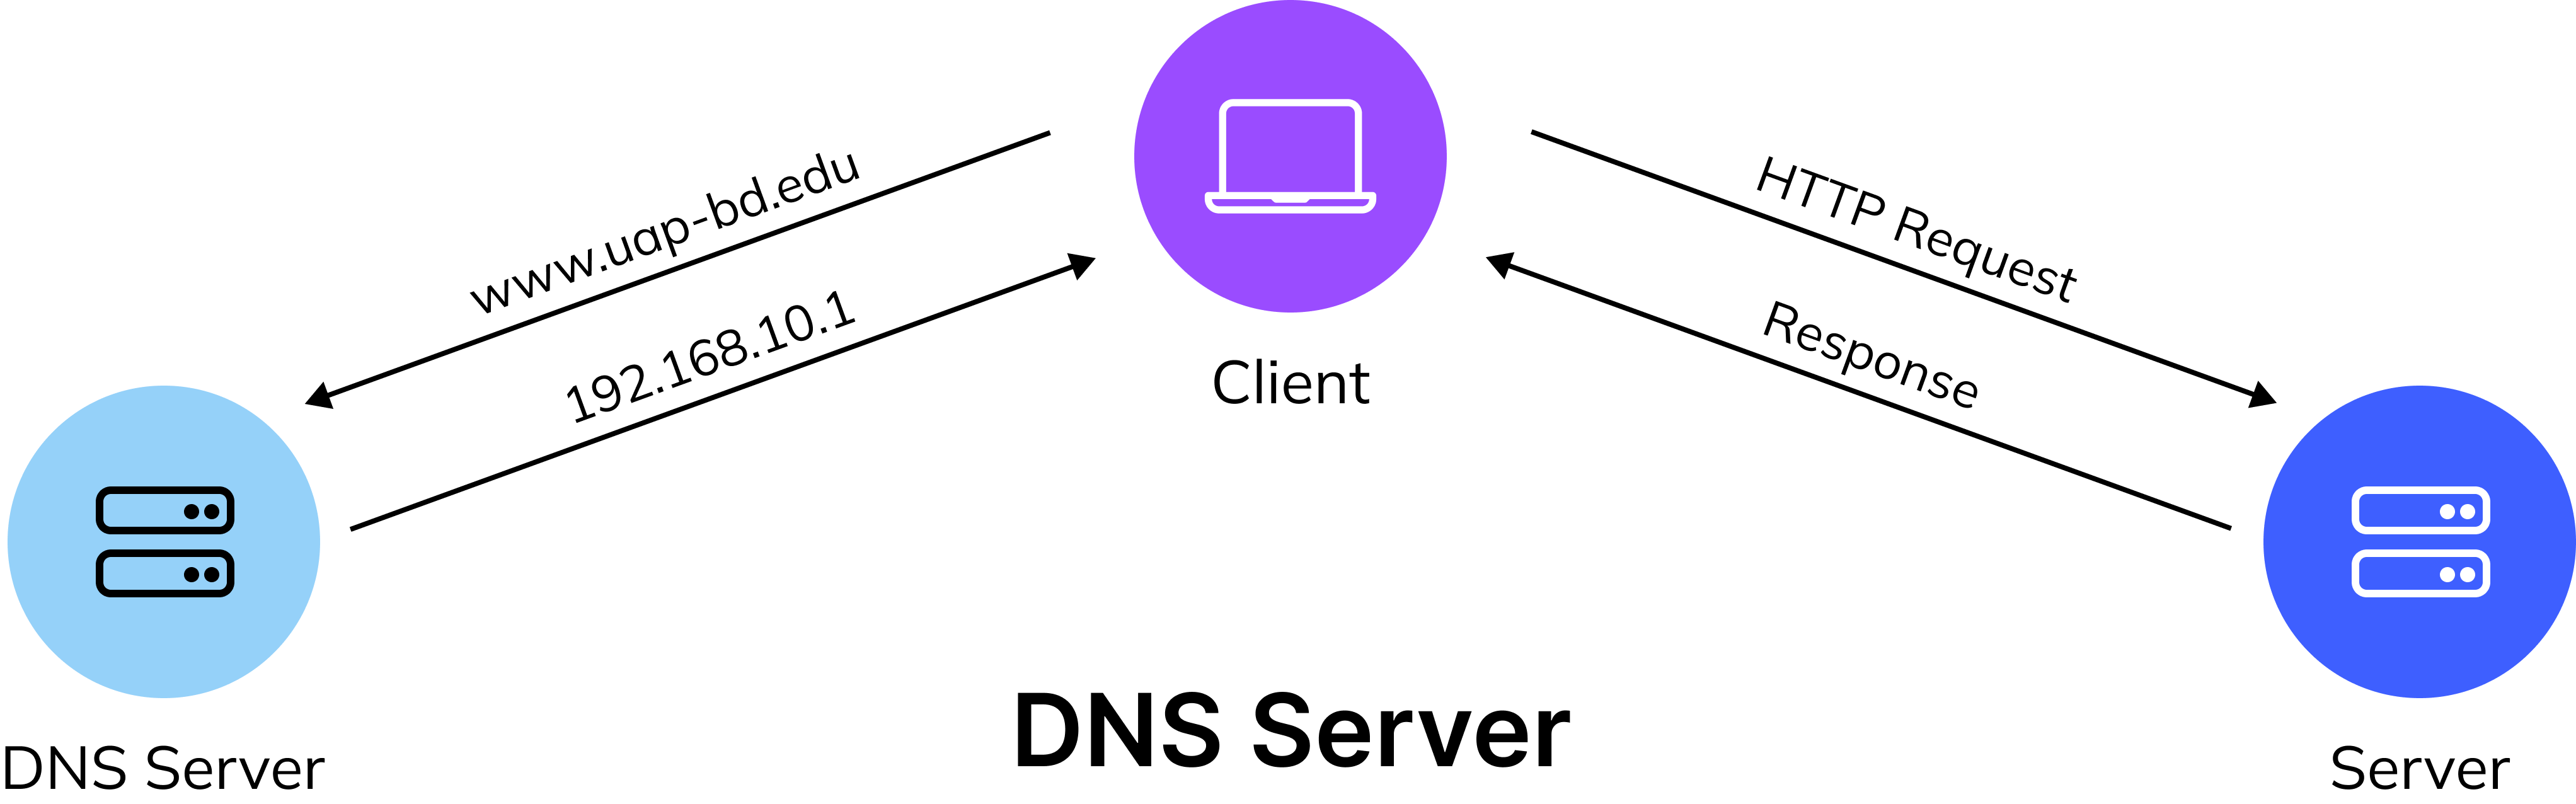
\includegraphics[width=0.6\linewidth]{figures/DNS.png}
\end{figure}


\section{DHCP (Dynamic Host Configuration Protocol):}
Automatically assigns IP addresses and network configuration parameters to devices on a network. It simplifies the process of network configuration and management for both users and administrators. DHCP is an application layer
protocol.

\begin{figure}[H]
   \centering
   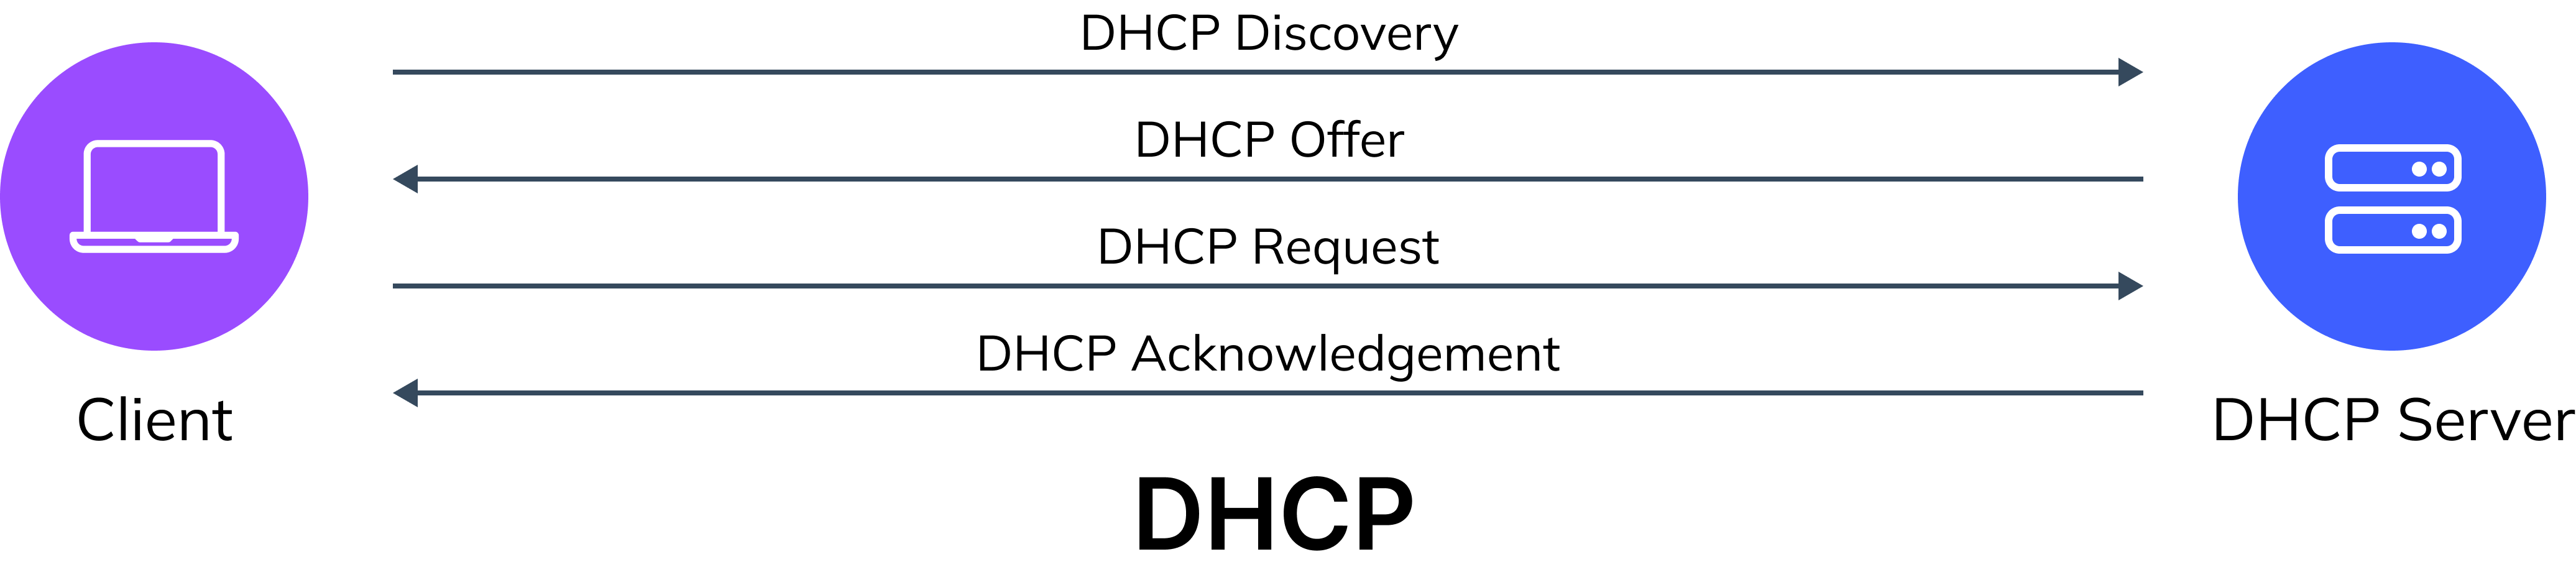
\includegraphics[width=0.6\linewidth]{figures/DHCP.png}
\end{figure}



\section{Comparison of Common Application Layer Protocols}

\begin{tabularx}{\textwidth}{|l|X|l|X|l|l|l|}
\hline
\textbf{Protocol} & \textbf{Stateful/Stateless} & \textbf{Transport Protocol} & \textbf{Persistent} & \textbf{Port No.} & \textbf{Data Transfer} \\
\hline
DNS  & Stateless (usually) & UDP & Non-persistent & 53  & In-band \\
\hline
HTTP & Stateless (default),\newline Stateful with cookies & TCP & Persistent & 80, 443 & In-band \\
\hline
SMTP & Stateful & TCP & Persistent & 25 & In-band \\
\hline
POP3 & Stateful & TCP & Persistent & 110 & In-band \\
\hline
FTP  & Stateful & TCP & Persistent & 21 (control), 20 (data) & Out-of-band \\
\hline
\end{tabularx}